\section{Perception Action paradigm}
The perception--action (PA) paradigm has a very strict connection with the definition of our searching algorithm. Lets try to understand what this paradigm is.

\subsection{The basic paradigm}
A PA map consider an agent in which external stimuli derive from a sensor network, that perform the perception section of the agent. Perception is therefore translated into a symbol that could be handled by the action section of the agent.
\begin{figure}[h]
\caption{Classical percetion--action map}
\centering
\begin{tikzpicture}[auto, node distance=2cm,>=latex']
	\node[input] (input) {};
	\node[block,right of=input] (perception) {Perception};
	\node[block,right of=perception] (action) {Action};
	\node[output, right of=action] (output) {};

	\draw[->] (input) -- node[pos=0.2] {Sensors} (perception);
	\draw[->] (perception) -- (action);
	\draw[->] (action) -- node[pos=0.7] {Actuators} (output);
\end{tikzpicture}
\end{figure}

Making a straight example on our device: we consider as sensor elements our digital ARTVA; the input to the perception stage, should be analyzed to perform an action, that is the movement of the drone towards buried position.

The relationship between the agent and the environment is called \emph{situatedness}, while the intercourse within what represents the \emph{body} on what represents the \emph{mind} of the agent is called \emph{embodiment}, as explained in \citep{thedynamicsofactivecaterogicalperception}.
\begin{marginfigure}
\centering
\begin{tikzpicture}[auto, node distance=1cm,>=latex']
	\node [rectangle, draw=black, minimum width=5cm,minimum height=3cm] (envir) {};
	\node [rectangle, draw=black, minimum width=3cm,minimum height=2.25cm] (body) at ++(0.75cm,-0.25cm) {};
	\node [rectangle, draw=black, dashed, minimum width=1.5cm,minimum height=1.5cm] (body) at ++(1.25cm,-0.5cm) {};
	\node [rectangle, fill=white] (situatedness) at ++(-0.75cm,-0.65cm) {$\underset{situatedness}{\longleftrightarrow}$};
	\node [rectangle, fill=white] (embodiment) at ++(.5cm,-0.85cm) {$\underset{embodiment}{\longleftrightarrow}$};
	\node [rectangle, fill=white, draw=black] at ++(-1.25cm,1.5cm) {\textbf{Environment}};
	\node [rectangle, fill=white, draw=black] at ++(1.5cm,0.85cm) {\textbf{Agent}};
	\node at(-0.3cm,0.6cm) {Body};
	\node at(1cm,0cm) {Mind};
\end{tikzpicture}
\caption{Embodiment and situatedness}
\end{marginfigure}

\subsection{Exploiting more complex behavior}
\myparagraph{Expanding PA}
Apart the basic behavior, the advantages of PA maps are related too the implementation of extremely complex actions using other techniques such as:
\begin{itemize}
\item subsumption and grounding
\item innate knowledge
\item bootstrapping
\item historical knowledge
\item shared knowledge
\end{itemize}
All those element could be serially implemented, one after the other, while they run together to create a coherent attitude with respect to the problem. One of the advanced feature that we will use in this project is the subsumption and the grounding of the symbols.

\myparagraph{Subsumption and grounding}
The \emph{symbols grounding} is an implementation of the embodiment of the agent as a stacked architecture in which different layer (subsumption), that performs different operations, are piled up in such a way that higher level, of higher complexity, could transparently use lower levels (symbols grounding \citep{harnad1990symbolgrounding}), and incorporate them to reach more complex behavior.
\begin{marginfigure}
\begin{tikzpicture}[auto, node distance=2cm,>=latex']

	\matrix [draw=white, row sep=0.1cm, column sep=1.5cm] {	
	   	& \node [block, right, anchor=west, text width=1.5cm, minimum width=1.5cm] (levelD) {Level 3}; & \\
		& \node [block, right,anchor=west, text width=1.8cm, minimum width=1.8cm] (levelC) {Level 2}; & \\
	 	& \node [block, right,anchor=west, text width=2.1cm, minimum width=2.1cm] (levelB) {Level 1}; & \\
		\node [input,right] (input) {}; & \node [block,anchor=west, text width=2.4cm, right, minimum width=2.4cm] (levelA) {Level 0}; & \node[output](output){} ; \\
 	};

	\draw [->] (input) -- node[below](mid) {Sensors} (levelA);
	\draw [->] (mid) |- node {} (levelB);
	\draw [->] (mid) |- node(midU) {} (levelC);
	\draw [->] (mid) |- node (midUb)  {} (levelD);
	\draw [->] (levelA) -- node[below] (midA) {Actuators} (output);
	\draw [->] (levelB) -| node[pos=0.3] (midB) {} (midA);
	\draw [->] (levelC) -| node[pos=0.3] (midC) {} (midB.south);
	\draw [->] (levelD) -| node[pos=0.3] (midD) {} (midC.south);

	\draw [->,dashed] (midUb.south) -- node  {} ++(0,0.8);
	\draw [<-,dashed] (midD.south) -- node {} ++(0,0.8);
\end{tikzpicture}
\caption{Subsumption and grounding architecture}
\end{marginfigure}

As an example, the very basic level that could be implemented is a stabilization control, that could be used to keep the plant in a controllable state. From this layer, an upper tracking layer will try to reduce the input error using the lower layer to preserve a safe stability for the system.

This techniques, introduced in \citep{layeredmobilerobot}, will be used in our avionics definition.

\myparagraph{Innate knowledge and emulation}
Evolution and generalization of the map are referred to the embodiment, with the implementation of an innate knowledge, that may be used to perform an internal emulation of the perceived environment. A typical example of this is the co--driver model implemented in \citep{artificialcodriver}, where emulation, defined as a mathematical model, is used to infer driver actions.

This techniques is also implemented in our avionics.
\begin{figure}[h]
\centering
\caption{Emulation in an agent}
\forceversofloat
\begin{tikzpicture}[auto, node distance=2.7cm,>=latex']
	% EMULATION
	\matrix[draw=black, row sep=0.1cm, column sep=0.2cm] (emulator) {
	 \node {\scriptsize{Model}}; \\ 
	 \node {\scriptsize{Hypothesis}};  \\
	};
	\node[above of=emulator] at ++(0,-1.8cm) {Emulator};

	% GROUNDING
	\matrix [draw=black,minimum width=4cm, minimum height=2.5cm, row sep=0.1cm, column sep=1cm, above of=emulator] (grounding) at ++(0,0cm) {	
		& \node [block, right,anchor=west, minimum width=1cm ,minimum height=0.5cm] (levelC) {}; & \\
	 	& \node [block, right,anchor=west, minimum width=1.25cm ,minimum height=0.5cm] (levelB) {}; & \\
		\node [input,right] (input) {}; & \node [block,anchor=west, right, minimum width=1.5cm, minimum height=0.5cm] (levelA) {}; & \node[output](output){} ; \\
 	};
	\node[above of=grounding] at ++(0,1.5cm) {Grounding};

	% EMULATOR
	\node[block,below of=emulator] (environment) at ++(0,1.2cm) {\textbf{Environment}};


	\draw [->] (input) -- node[below](mid) {} (levelA);
	\draw [->] (mid) |- node (midK) {} (levelB);
	\draw [->] (mid) |- node(midU) {} (levelC);
	
	\draw [->] (levelA) -- node[below] (midA) {} (output);
	\draw [->] (levelB) -| node[pos=0.3] (midB) {} (midA);
	\draw [->] (levelC) -| node[pos=0.3] (midC) {} (midB.south);


	\draw [->,dashed] (mid) -- node  {} ++(0,1.8);
	\draw [<-,dashed] (midC.south) -- node {} ++(0,0.5);

	\node[right of=grounding] (gr) {};
	\node[left of=grounding] (gl) {};

	\draw [->] (emulator.west) -|  (gl.south) |- (grounding);
	\draw [<-] (emulator.east) -|  (gr.south) |- (grounding);

	\node[block,minimum width=6cm, minimum height=5.25cm,dashed] (agent) at ++(0,1.9cm) {};
	\node[above of=agent] at ++(0,2cm) {\textbf{Agent}};

	\draw [<-] (environment.east) -- ++(2.5cm,0) |- (grounding);
	\draw [<-] (environment.west) -- ++(-2.5cm,0) |- (grounding);

\end{tikzpicture}
\end{figure}

\myparagraph{Bootstrapping and more}
In this paragraph, for completeness, we could cite other techniques that generalize embodiment and situatedness. One of the most recent generalization approach is called \emph{bootstrapping}. From \citep{sun2001implicit} and \citep{hierarchicalbootstrapping}, a cognitive system should identify and define its motion primitives\marginnote{Even if this procedure is clearly different from innate knowledge, the implementation of this technique do not exclude the implementation of some kind of innate knowledge.}. 

The exploration of motion domain is performed through the use of random inputs and fuzzy logic\citep{aframeworkforhierarchicalperceptionaction} on perception:
\begin{itemize}
\item random exploration gives an initial model for the primitives
\item repetition on the primitives allows the system to remove redundancies
\item further repetition remove unused parameters
\item last repetitions allows to perform an optimization and update of the model parameters
\end{itemize}

\section{Building the PA map of the drone}

\subsection{Overview of our searching map}

In figure \ref{fig:genPAmap} a comprehensive version of the map is presented. The map shows a tri--dimensional evolution in the upper side, where two different aims are achieved. One one side we have the searching for the signal, and on the other side we have the searching for the signal source. This particular design in the map was implement to grant to the avionics the ability to perform a sort of reasoning and reach a multiple objective, as it will be explained later on.

The drone has a complex control system, already implemented in IMU shield, that takes in consideration a linearized feedback that feeds an LQR control loop\citep{belanger1995control}. 

The system could be modified to solve a tracking problem, that will be used by the upper level. The tracking problem uses transparently the stabilization layer and it is used by the searching layer.

Upper layers, obstacle avoiding and altitude keeping, preserve drone to collide with isolated obstruction and at an altitude that is safe for rescuers. 
\begin{figure}[h]
	\centering
	%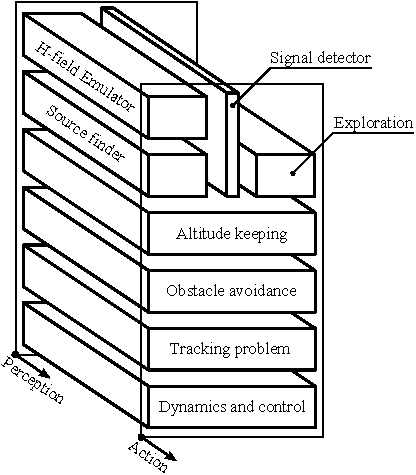
\includegraphics[scale=0.9]{ch3/img/PA_map_general.pdf}

	\begin{tikzpicture}[>=latex']
		\drawplanexy{-0.3}{-0.3}{-0.3}{6.7}{10}{dashed}{perception}
		\node [at=(perception_D),xshift=30,yshift=-10] {\textbf{Perception}};
		\drawcube{0}{0}{5}{6.4}{1}{white}{dinamica}{Dynamics and control}{};
		\drawcube{0}{1.2}{5}{6.4}{1}{white}{tracking}{Tracking Problem}{};
		
		\drawcube{0}{2.4}{5}{6.4}{1}{white}{ostacoli}{Obstacle Avoidance}{};
		\drawcube{0}{3.6}{5}{6.4}{1}{white}{altitude}{Altitude Keeping}{};
		
		\drawcube{0}{4.8}{5}{3}{1.5}{white}{source}{Source searching}{text width=2cm,align=center};
		\drawcube{0}{6.5}{5}{3}{1.5}{white}{emulatore}{Emulation}{text width=2cm,align=center};

		\drawplanezy{3.2}{4.8}{5}{4.5}{radar_det}{fill=white,opacity=0.90}{Radar detect}{rotate=45,xslant=1};

		\drawcube{3.4}{4.8}{5}{3}{3.2}{white}{alpha}{Exploration routines}{text width=2cm,align=center};
		\drawplanexy{-0.3}{-0.3}{5.3}{6.7}{10}{dashed}{action}
		\node [at=(action_D),xshift=20,yshift=-10] {\textbf{Action}};

		\draw [->,line width=1.5] (action_D) -- ++(0,0,2);
		\draw [->,line width=1.5] (perception_D) -- ++(0,0,2);

		\coordinate [at=(radar_det_D), yshift=-20] (arrows_point);
		\draw [->,dashed]  (arrows_point) -- ++(1.5,0,0); 
		\draw [->,dashed]  (arrows_point) -- ++(-1.5,0,0); 
	\end{tikzpicture}
	\forcerectofloat
	\caption{General Perception--Action map for our drone}
	\label{fig:genPAmap}
\end{figure}
\FloatBarrier